\documentclass{beamer}
\usepackage[utf8]{inputenc}
%\usetheme[secheader]{Boadilla}
\usetheme{Malmoe}

\definecolor{chameleongreen1}{RGB}{64,64,64}
\definecolor{chameleongreen2}{RGB}{131,131,131}
\definecolor{chameleongreen3}{RGB}{99,99,99}
\definecolor{chameleongreen4}{RGB}{0,0,0}

\setbeamercolor*{palette primary}{fg=white,bg=chameleongreen1}
\setbeamercolor*{palette secondary}{fg=white,bg=chameleongreen2}
\setbeamercolor*{palette tertiary}{fg=white,bg=chameleongreen3}
\setbeamercolor*{palette quaternary}{fg=white,bg=chameleongreen1}

\setbeamercolor*{titlelike}{bg=chameleongreen1,fg=white}
\setbeamercolor*{frametitle}{bg=white,fg=chameleongreen1}
\setbeamercolor*{part title}{bg=white,fg=chameleongreen1}
\setbeamercolor*{item}{fg=chameleongreen1}

\setbeamercolor*{separation line}{}
\setbeamercolor*{fine separation line}{}
\useinnertheme[shadow=true]{rounded}

\setbeamercolor{section in toc}{fg=black,bg=white}
\setbeamercolor{item projected}{fg=white}

\addtobeamertemplate{footline}{\hfill\insertframenumber/\inserttotalframenumber\hspace{2em}\null}


\title{Fire Monkeys\\ Modélisation de feu en temps réel}
\author{Benjamin Aupetit - Julien Champeau - Arnaud Emilien}
\date{Jun 14 2010}

\begin{document}

%% 0 - Présentation de l'équipe
\begin{frame}
   \titlepage
\end{frame}

%% 1 - Présenter le plan de la présentation
\begin{frame}
  \tableofcontents
\end{frame}

% 2 - Expliquer l'objectif :
%    Réaliser un modèle de combustion d'objets en 3D temps réel.
\section{Objectif}
\begin{frame}{Objectif}
  Réaliser un modéle de combustion d'objets en 3D temps réel.\\
  \textbf{image}
  \begin{itemize}
    \item{Le feu}% flamme réaliste visuellement.
    \item{La fumée}% comportement réaliste.
    \item{Iteraction avec des objets}% gérer les collisions entre le feu et les objets
    \item{Propagation sur l'objet}% propagation du feu sur un objet
    \item{Combustion d'objet}% destruction de l'objet par le feu
  \end{itemize}
\end{frame}

\begin{frame}{Les étapes de notre démarche}
  \begin{itemize}
  \item{découvrir le milieu scientifique} % domaine de recherche
  \item{étudier différents articles} % étude du sujet
  \item{Concevoir notre propre modèle} % comprehension des article et choix d'une solution
  \item{Implémenter le modèle} % sur CPU
  \item{Améliorer le modèle} GPU ( objectif initial ) %
  \end{itemize}
\end{frame}

\section{Le modèle}
\begin{frame}{Modèle d'intéraction}
  Interractions entre le modèle de feu et le modèle d'objet.
  \begin{itemize}
  \item Présence des objets ( i.e. : pas de flamme a l'interieur des objets )
  \item Transimission des informations de chaleur d'un modèle à l'autre.
  \item Gestion de la ``pyrolise'' des objets.
  \end{itemize}
\end{frame}

\subsection{Le fluide}
\begin{frame}{Principe}
  \begin{itemize}
  \item Modèle basé sur le travail de \textbf{Jos Stam}, notemment
    \textbf{Stable Fluids}(SIGGRAPH 99 Conference Proceedings).
  \item Résolution de manière approchée des équation de Navier-Stokes
    pour la dynamique des fluides icompréssibles.
  \item Un rendu utilisant le principe de ``BillBoard''.    
  \end{itemize}
\end{frame}

\begin{frame}{La diffusion}
  La diffusion représente la capacité du fluide à se déplacer dans le
  milieu ambiant.
  \begin{figure}[h]
      \begin{equation}
        \frac{\partial \vec{u}}{\partial t} =  \nu{\nabla^2}\vec{u} 
      \end{equation}
      \caption{Equation de diffusion}
      \label{DiffusionEquation}
  \end{figure}
\end{frame}

\begin{frame}{Diffusion}
  \begin{figure}[h]
    \centering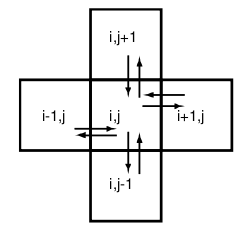
\includegraphics[scale=0.6]{STAM.png}
    \caption{Diffusion sur une grille 2D}
    \label{DiffusionStam}
  \end{figure}
\end{frame}


\begin{frame}{L'advection}
  Le champ de vitesse va servir à transporter la quantité de fluide
  dans l’espace. L’auto-advection du champ de vitesse est ce qui va
  permettre le mouvement des particules de gaz dans le milieu.
  \begin{figure}[h]
    \centering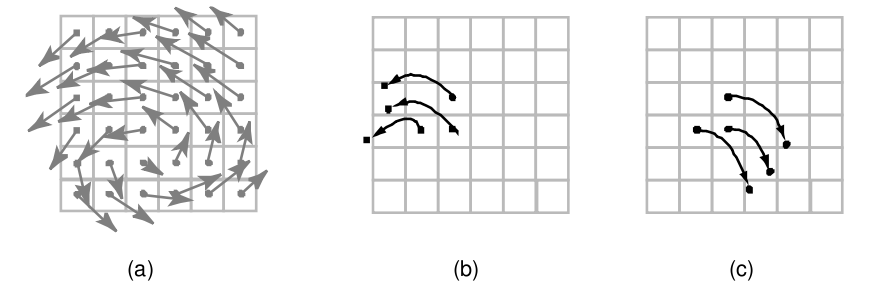
\includegraphics[scale=0.6]{STAM2.png}
    \caption{Principe de l'advection évoquée par \textbf{Jos Stam}}
    \label{AdvectionStam}
  \end{figure}
\end{frame}

\begin{frame}{La projection}
%image
\end{frame}

\begin{frame}{Le rendu}
%image + perlin
\end{frame}

\subsection{Les objets}
\begin{frame}{Une représentation par voxel}
%image + champ de distance + isosruface + marching cube adaptatif
\end{frame}

\begin{frame}{Combustion de l'objet}
%localite du marching cube
\end{frame}

\section{Portage du modèle de fluide sur GPU}
\begin{frame}{Le calcul sur GPU}
\end{frame}

\begin{frame}{Principe de fonctionnement}
\end{frame}

\begin{frame}{Les problèmes rencontrés}
\end{frame}

\begin{frame}{Réalisations}
\end{frame}

\section{Démonstration}
\begin{frame}
  \begin{center}
    \textbf{Démonstrations}
  \end{center}
\end{frame}

\section{Conclusion}
\begin{frame}{Conclusion}
\end{frame}

\begin{frame}{Remerciements}
  \begin{itemize}
  \item{Marie-Paule Cani} pour avoir accepté de nous encadrer, pour
    ses conseils et indices de recherche.
  \item{Cyril Crassin} pour nous avoir aidé à comprendre le
    fonctionnement de GLSL.
  \item{Aurelie Catel} pour le suivi de gestion de projet.
  \item{Nintendo\texttrademark} pour Super Smash Bross Melee ©.
  \end{itemize}
\end{frame}

\end{document}

